\section{Introduction}
\label{sec:introduction}


The main objective of this laboratory assignment is to analyse a circuit using a simulation and the node and mesh methods. It is important to rely on a method that simplifies a circuit as it gives us many information. So, it is equally important to understand if these methods can be applied and if the results are satisfactory. To prove the truthfulness of this analysis, the following report was developed. The circuit can be seen in Figure~\ref{fig:circuit}.

In the next section (~\ref{sec:analysis}), we briefly explain the procedure to analyse the given circuit, first with the node method and then with the mesh method. In order to solve the necessary calculations and obtain the values for the tension and current in every node and branch, respectively, we used Octave maths tool.
Then, we resorted to Ngspice to simulate our circuit and obtain the simulated values for the same physical quantities previously calculated. These values will be shown in Section~\ref{sec:simulation}. We will also compare both results and give certain notes related to our analysis.
The report finishes with its conclusion, in section~\ref{sec:conclusion}, where we resume the most important points of the lab assignment.


\begin{figure}[h] \centering
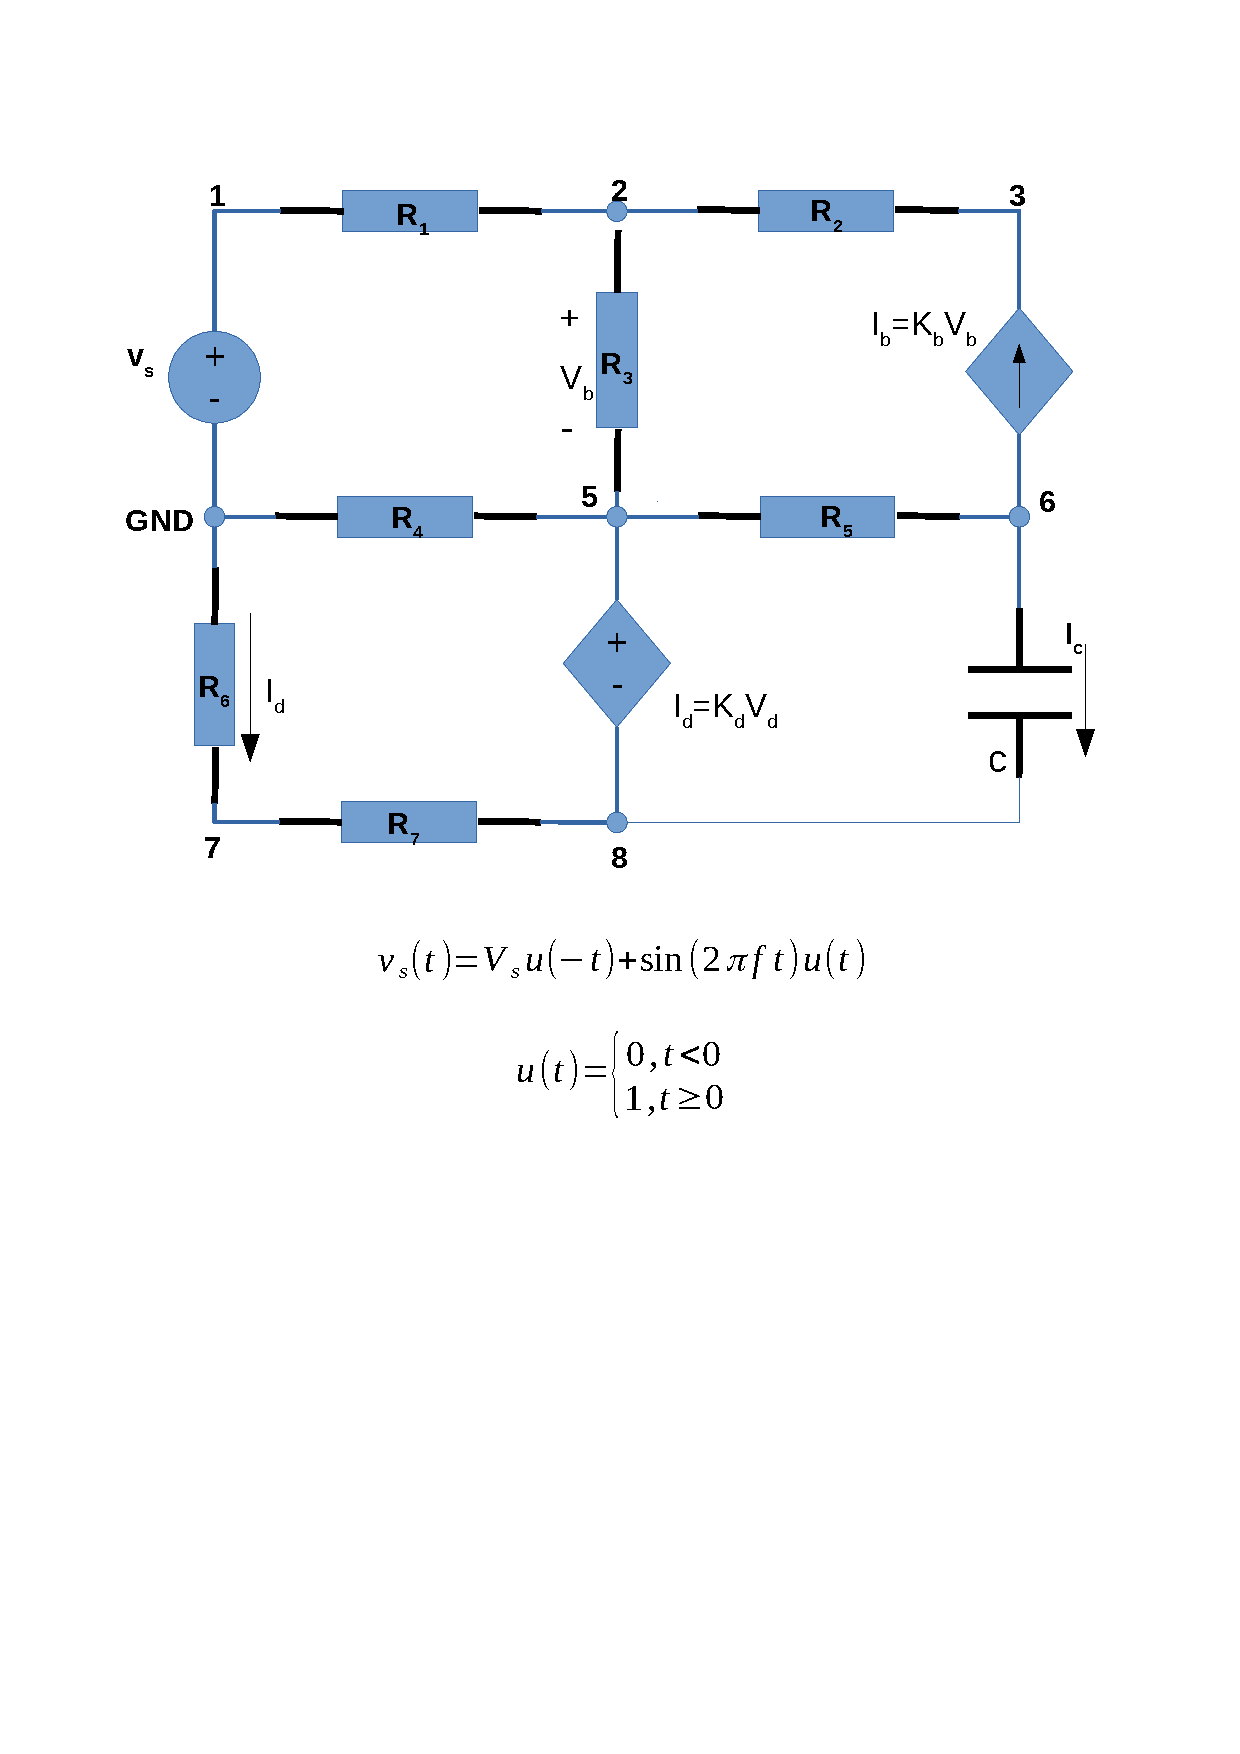
\includegraphics[width=0.6\linewidth]{circuit.pdf}
\caption{Circuit under analysis.}
\label{fig:circuit}
\end{figure}




